\documentclass[11pt,a4paper]{article}
\usepackage{fontspec}
\usepackage{polyglossia}
\setmainlanguage{english}
\setotherlanguage{ukrainian}
\setmainfont{cmunrm.otf}[Path=fonts/,BoldFont=cmunbx.otf,ItalicFont=cmunti.otf,BoldItalicFont=cmunbi.otf]
\setsansfont{cmunss.otf}[Path=fonts/,BoldFont=cmunsx.otf,ItalicFont=cmunsi.otf,BoldItalicFont=cmunso.otf]
\setmonofont{cmuntt.otf}[Path=fonts/,ItalicFont=cmunit.otf]
\newfontfamily\cyrillicfont{cmunrm.otf}[Path=fonts/,BoldFont=cmunbx.otf,ItalicFont=cmunti.otf,BoldItalicFont=cmunbi.otf,Script=Cyrillic]
\newfontfamily\cyrillicfontsf{cmunss.otf}[Path=fonts/,BoldFont=cmunsx.otf,ItalicFont=cmunsi.otf,BoldItalicFont=cmunso.otf,Script=Cyrillic]
\newfontfamily\cyrillicfonttt{cmuntt.otf}[Path=fonts/,ItalicFont=cmunit.otf,Script=Cyrillic]
\usepackage[a4paper,margin=25mm]{geometry}
\usepackage{microtype}
\usepackage{booktabs,longtable,tabularx,array,multirow}
\usepackage{graphicx}
\graphicspath{{../figures/}}
\newcolumntype{Y}{>{\raggedright\arraybackslash}X}
\usepackage{caption}
\captionsetup{font=small,labelfont=bf,labelsep=colon,justification=justified,singlelinecheck=false}
\captionsetup[table]{position=top}
\usepackage{enumitem}
\usepackage{amsmath}
\usepackage{float}
\usepackage{placeins}
\usepackage[numbers,sort&compress]{natbib}
\usepackage{xurl}
\usepackage{hyperref}
\urlstyle{same}
\hypersetup{hidelinks,pdfencoding=auto,unicode=true,pdftitle={Social: An Evidence-Grounded Framework for Automated Social Conflict and Information Incident Analysis},pdfauthor={Oleksandr Pylypenko}}
\emergencystretch=2em
\setlist{nosep,leftmargin=1.5em}
\renewcommand{\arraystretch}{1.12}
\renewcommand{\bibfont}{\small}
\setlength{\bibsep}{2pt}

\DeclareRobustCommand{\code}[1]{\nolinkurl{#1}}
\newcommand{\baseline}{\texttt{f0e9d0d}}
\begin{document}
\begin{center}
{\LARGE Social: An Evidence-Grounded Framework for Automated Social Conflict and Information Incident Analysis\par}
\vspace{0.4em}
{\large Architecture, Implementation, Evaluation, and Lessons from a Real-World Case\par}
\vspace{0.8em}
{\large Oleksandr Pylypenko\par}
{\small Independent Researcher in Artificial Intelligence and Machine Learning\par}
{\small PhD Student, State University of Trade and Economics, Kyiv, Ukraine\par}
{\small ORCID: \href{https://orcid.org/0009-0004-9610-9242}{0009-0004-9610-9242}\par}
{\small \href{mailto:O.Pylypenko@knute.edu.ua}{\texttt{O.Pylypenko@knute.edu.ua}}\par}
\vspace{0.4em}
10 November 2026
\end{center}
\begin{abstract}
Digital traces of social conflicts combine incomplete observations, repeated claims, contradictory accounts, and media whose publication time differs from recording or event time. Integrating these records requires automation that preserves evidentiary boundaries rather than generating a single confident narrative. This paper describes Social, a modular Python research system combining platform-specific collection, versioned snapshots, text-similarity and temporal analysis, evidence accounting, bounded retrieval, typed event organization, local media processing, and report quality gates. We audit a frozen implementation and distinguish implemented functions, structural tests, empirical checks, and unmeasured semantic properties. Evaluation reproduces an exhaustive 369-edge cross-channel text-similarity graph, finds 367 of these edges in the legacy MinHash output, recalculates 16 saved conditional-randomization summaries, and reproduces a 25-draw prefix for each of four null models. A fresh offline suite passes 783 tests and 16 subtests. These results establish bounded computational reproducibility, not factual accuracy. The current curated 25-claim package emits 19 supported-within-scope and six insufficient-evidence states, but targeted challenges expose numeric-predicate and negation errors in its relation heuristics. A disclosed post-audit rule revision removes all 36 wrong-predicate and negation acceptances in an authored 534-case stress test and changes the package to 18 supported and seven insufficient-evidence states; this stress test is not an accuracy estimate. The general offline workflow conservatively retains retrieved claims as unverified and requires separately supplied report inputs. Historical media receipts document 607 decodable assets; an 18-clip supplied-reference comparison yields 44.58\% micro word error rate without independently established reference-review provenance. A real-world application illustrates integration and coverage limitations. Social's contribution is an inspectable analytical workflow and explicit account of its reliability boundaries, rather than a new inference algorithm or validated autonomous investigator.
\end{abstract}
\noindent\textbf{Keywords:} computational social science; crisis informatics; evidence provenance; automated analysis; information dynamics; research software; uncertainty.

\section{Introduction}
Social conflicts increasingly generate parallel records in channels, comment threads, news reports, institutional statements, and short audiovisual fragments. These records support several different analytical tasks: documenting what a source said, tracing how a claim circulated, identifying a repeated text, organizing candidate events, and assessing whether available evidence supports an allegation. A system that conflates these tasks can turn a plausible narrative into an apparently verified account. A copied statement is not a new witness, a publication timestamp is not a recording timestamp, and a statistical departure from a timing model does not identify an organizer.

Crisis informatics has long emphasized the difficulty of extracting useful information from heterogeneous and noisy social-media streams \citep{imran2015crisis}. Computational social science adds concerns about platform access, sampling, measurement, and ethics \citep{Olteanu2019,VicentePaula2023}. Digital open-source investigation requires preservation and contextual verification of materials, including explicit treatment of uncertainty \citep{berkeleyProtocol2022}. These requirements become particularly important when software combines traditional analysis with generative AI. Fluent synthesis can hide uncertainty rather than resolve it; even citation-bearing generation requires separate assessment of whether citations support the text \citep{gao2023alce}.

Social addresses this integration problem as a research-software framework. Its practical objective is to help an analyst move from collected digital traces to inspectable intermediate records and bounded analytical outputs. The implementation contains platform-specific acquisition scripts, information-wave analysis, a linked evidence ledger, retrieval and verification rules, typed event processing, local media pipelines, and report validators. These components differ substantially in maturity, integration, and evaluation. Describing them as one uniformly autonomous investigator would obscure those differences.

This paper asks: \emph{How can a modular, evidence-grounded software system integrate heterogeneous digital traces to support automated analysis of social conflicts and information incidents while preserving provenance, uncertainty, and reproducibility?} We study an existing implementation rather than propose a new algorithm. The analysis freezes a Git revision, inspects execution paths, reconciles numerical artifacts, reruns bounded computations, and deliberately tests semantic failure cases. The Petropavlivska Borshchahivka application supplies realistic workloads, but is not an independent test of generalization. A separate project manuscript studies that incident itself \citep{pylypenko2026case}; the present paper examines the software and its evidentiary boundaries.

\subsection{Contributions of this work}
The contributions are fourfold. First, we provide a code-grounded integration map that separates reusable processors, platform collectors, experimental heuristics, curated case builders, and report-generation scripts. Second, we describe the implemented evidence model and the distinction between technical provenance, information lineage, source independence, and semantic validity. Third, we report reproducibility checks for similarity detection, conditional randomization, structural contracts, and a bounded offline workflow. Fourth, we expose concrete semantic counterexamples, measure a disclosed rule revision against them, and define the limits of the system's demonstrated autonomy. These contributions support more accountable use and evaluation of analytical software; they do not establish a new state of the art in fact verification, event extraction, or attribution.

\section{Related work}
\label{sec:related}

Social intersects crisis informatics, news-event databases, automated claim
verification, retrieval-supported generation, and digital investigation practice.
These traditions address different units: messages, reported events, claims,
answers, or preserved media. Their outputs therefore require different validation.
A retrieved article may be relevant without supporting a claim; several reports
may share one origin; and a decoded video may remain unverified as to location,
time, or interpretation. We use this distinction to position the inspected
software, rather than treating adjacent systems as interchangeable competitors.
Table~\ref{tab:related} summarizes their documented purposes and comparison limits.

Crisis informatics provides the immediate problem setting. Imran et
al.~\cite{imran2015crisis} organize emergency-message processing around filtering,
classification, ranking, aggregation, extraction, and summarization. This framing
connects heterogeneous collection with the analyst's need to reduce information
overload. Social adopts a similar workflow perspective but studies a bounded
incident reconstruction and its inspectable artifacts. Its platform panels and
case-specific selection rules do not constitute a representative population
sample. Successful execution of a filter or collector consequently cannot
establish completeness, situational accuracy, or usefulness to emergency
responders without a separate evaluation of those outcomes.

News-event infrastructures show that organizing observations into events is an
established task. GDELT separates CAMEO-coded event records from news mentions and
provides extraction confidence and geographic attributes; its GKG supplies
document-level entities, themes, and contextual
metadata~\cite{gdelt2015events,gdelt2015gkg}. ACLED uses researcher coding and a
defined political-disorder taxonomy, with explicit date and location precision
and source information~\cite{acledCodebook}. Event Registry groups multilingual
news articles, extracts event attributes, and supports event search and
exploration~\cite{leban2014eventregistry}. These works motivate explicit event
units and distinctions between reports and occurrences. Social does not claim
novelty for extraction or clustering. Its narrower research question concerns
how capture receipts, evidence passages, claim assessments, and event hypotheses
can remain inspectably connected within a bounded investigation.

Automated fact-checking introduces a complementary requirement: evaluate the
evidence as well as the predicted judgment. FEVER combines claims derived from
Wikipedia with evidence selection and supported, refuted, or insufficient-information
labels~\cite{thorne2018fever}. AVeriTeC addresses real-world claims using web
evidence, question--answer decompositions, and justifications, explicitly attending
to temporal leakage and evidence sufficiency~\cite{schlichtkrull2023averitec}.
InFact implements a staged, retrieval-based LLM fact-checking
pipeline~\cite{rothermel2024infact}. These are relevant task formulations and
evaluation precedents. Social's contract checks and incident regressions do not
amount to a FEVER or AVeriTeC benchmark result, and no accuracy ranking against
these systems is implied. Claim-level correctness and reconstruction quality
remain separate from software integration success.

Retrieval-augmented generation combines learned generation with external
retrieved memory~\cite{lewis2020rag}. ALCE makes citation quality a distinct
evaluation dimension alongside correctness and
fluency~\cite{gao2023alce}. This distinction matters for generated investigation
reports: a syntactically present citation is not necessarily relevant, sufficient,
or faithful to the associated sentence. Social's source and passage references
provide objects that can be inspected, while their existence alone supplies no
guarantee of semantic support. Neither retrieval relevance nor a model's verbal
confidence should be interpreted as an independently calibrated probability that
an incident claim is true.

Diffusion observatories and media-verification tools address further parts of
the workflow. Hoaxy tracks the circulation of URLs from monitored sources and
their fact-checking counterparts; its 2016 description explicitly distinguishes
tracking from performing fact checking~\cite{shao2016hoaxy}. InVID and WeVerify
combine keyframe extraction, reverse-image search, metadata inspection, forensic
assistance, and guided analyst tools~\cite{invidVerificationPlugin,weverifyVerificationPlugin}.
They establish substantial prior art for integrated verification assistance.
Their documented functions do not make every diagnostic result a factual
verdict. Likewise, Social's local media indexing and candidate transcripts must
be distinguished from independent authentication and source-context verification.

The Berkeley Protocol separates collection, preservation, verification,
investigative analysis, and reporting within a professional and ethical
investigation process~\cite{berkeleyProtocol2022}. It is methodological guidance,
not a software certification. Research-software practices concerning organized
data, documented transformations, version control, and reproducible workflows
provide a complementary engineering frame~\cite{wilson2017practices}. Social's
contribution is assessed against concrete implemented artifacts and bounded
checks within these established traditions. Neither adopting a terminology nor
passing local tests establishes protocol compliance, evidentiary admissibility,
universal platform coverage, or semantic validity across incidents. Those broader
claims require additional evidence and an evaluation design matched to them.

\begin{table*}[t]
\centering
\footnotesize
\setlength{\tabcolsep}{3pt}
\renewcommand{\arraystretch}{1.12}
\caption{Qualitative positioning from the cited primary sources and the present
code audit. Cells describe documented functions or validation scope, not measured
superiority. Historical papers and tool pages do not establish current platform
access.}
\label{tab:related}
\begin{tabularx}{\textwidth}{@{}p{20mm}YYYYY@{}}
\toprule
System & Primary purpose & Provenance representation & Event reasoning & Uncertainty & Evaluation / comparison \\
\midrule
GDELT & News-event and contextual metadata & Event/mention identifiers; document links & CAMEO actions; contextual fields & Extraction confidence; geographic estimates & Codebook describes fields; no shared incident benchmark here \\
ACLED & Coded political-disorder events & Sources and event notes & Researcher-coded event taxonomy & Date/location precision; coding conventions & Methodology and review process; different observation unit \\
Event Registry & News-to-event organization & Associated news articles & Multilingual clustering and attributes & Language and clustering scope & 2014 system description; no common test here \\
Hoaxy & URL-sharing observatory & Monitored URLs and sharing observations & Circulation analysis & Selected sources and platform sample & Preliminary sharing analysis; no truth adjudication \\
InVID--WeVerify & Analyst media-verification assistance & Context, metadata and search results & Analyst-guided media examination & Diagnostic tools require interpretation & Official tool descriptions; no joint performance test \\
Social & Bounded incident evidence workflow & Capture hashes, paths, passages and typed links & Claim assessments; event hypotheses & Access states and unresolved evidence & Local regression/integrity checks; limited semantic validation \\
\bottomrule
\end{tabularx}
\end{table*}

\section{Research Objectives and Design Principles}
The audit operationalizes six research questions. \textbf{RQ1} asks which source and analytical components are actually integrated and where manual interfaces remain. \textbf{RQ2} asks which provenance invariants are enforced and what they fail to establish. \textbf{RQ3} asks whether similarity and conditional-randomization outputs reproduce on frozen inputs. \textbf{RQ4} concerns separation of communication timestamps, supplied physical-event intervals, and unknown time. \textbf{RQ5} asks which semantic failure modes survive software-level quality gates. \textbf{RQ6} asks which bounded analyst workflow is supported without implying independently validated investigation.

Three design principles organize the implementation. \emph{Typed separation} keeps sources, artifacts, statements, evidence assessments, and findings distinct. \emph{Explicit incompleteness} retains missing inputs, failed collection, unknown lineage, unresolved events, and unverified claims. \emph{Inspectable computation} records inputs, parameters, versions, and outputs so that an analyst can examine how a result arose. These principles are partly implemented and partly limited by legacy interfaces; they are not asserted as universal invariants across every script.

Our method is an implementation audit with bounded empirical checks. We prioritize current code and fresh computations over completion reports and plans. A successful test establishes only its tested property. An output count establishes inventory, not correctness. A curated example demonstrates a workflow, not blind accuracy. The new publication artifacts preserve these distinctions in a claim--evidence matrix and machine-readable experiment manifest. No core Social implementation or previous case-study manuscript was changed to improve results reported here.

\section{System Architecture}
\subsection{Audited implementation and component boundaries}
The system snapshot is commit \code{f0e9d0d67422b0c286a2cb9e7d4e935a833a9533}, dated 9 November 2026, on \code{codex/social-master-plan-audit-remediation}. The local \code{main} revision is older and omits relevant remediations. The audited worktree was clean before the new paper artifacts were created. Source, analysis scripts, tests, JSON schemas, data snapshots, research documents, and reports are stored in distinct directories. Social is not currently distributed through a unified package or dependency lockfile. Entry points are Python modules and research scripts rather than a single comprehensive application command.

Figure~\ref{fig:architecture} shows the implemented composition. Platform collectors and case-specific preprocessing produce snapshots for legacy information analysis. A newer typed branch links source captures to an evidence ledger and bounded analysis. Video indexing and extraction form a separate local pipeline; the general incident runner does not automatically invoke the full media pipeline. The controller integrates a fixed Source Watch adapter and optional pretyped offline inputs. It does not dispatch every collector, autonomously expand source discovery, or infer every intermediate object from raw records.

\begin{figure}[tbp]
\centering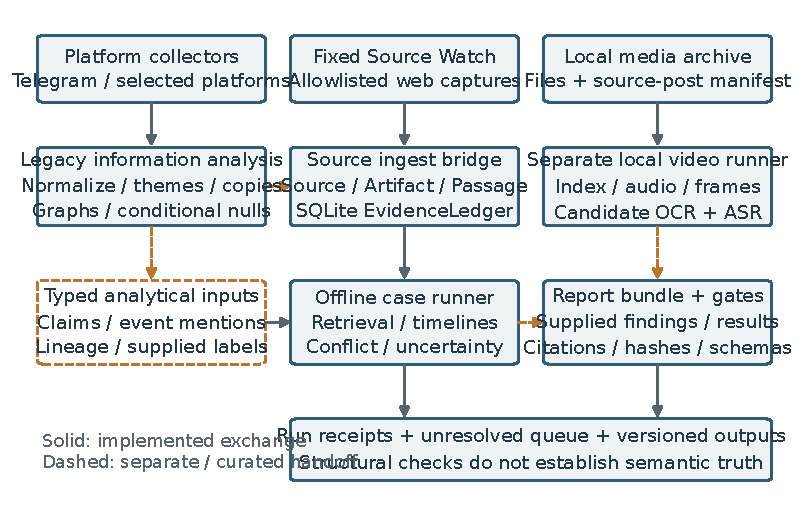
\includegraphics[width=\linewidth]{system_architecture.pdf}
\caption{Implemented Social components and integration boundaries at the audited revision. Solid arrows denote implemented exchanges; dashed arrows mark manual or separately executed adapters. The media and legacy-analysis branches are executable but are not all orchestrated by the general incident runner.}
\label{fig:architecture}
\end{figure}

\begin{table}[tbp]
\caption{System components: implementation and validation are separate dimensions. Paths are relative to the repository root; most analytical modules reside in \code{src/analysis/}.}
\label{tab:components}\small
\begin{tabularx}{\linewidth}{@{}p{25mm}X p{25mm}@{}}\toprule
Component & Concrete implementation and role & Evidence of readiness\\\midrule
Acquisition & \code{src/tg_collect.py}, \code{src/tg_comments_collect.py}, \code{src/source_watch_collect.py}; separate API/web collectors & Implemented; access-dependent, offline tests\\
Snapshot preparation & \code{build_continuation.py}, \code{prep.py}; verified merge and case relevance rules & Implemented; provenance checks; semantic relevance not independently validated\\
Information analysis & \code{analyze.py}, \code{coordination_lsh_audit.py}, \code{coordination_null_models.py} & Implemented; exact graph and bounded replay evaluated\\
Evidence accounting & \code{src/evidence_ledger.py}, \code{source_ingest_bridge.py}, \code{source_lineage.py} & Implemented; structural/reference tests\\
Evidence assessment & \code{claim_verification.py}; BM25, heuristics, aggregation & Retrieval implemented; semantic heuristics experimental\\
Events and conflict & \code{event_reconstruction.py}, \code{conflict_analysis.py}; supplied typed records & Implemented organization; physical truth not evaluated\\
Local media & \code{src/media_pipeline.py}, \code{video_pipeline_runner.py}, \code{media_fingerprints.py} & Implemented; technical receipts; semantic thresholds uncalibrated\\
Audience analytics & \code{audience_response.py}, \code{audience_aggregation.py} & Implemented contracts / aggregation; labels supplied, accuracy not evaluated\\
Workflow and reports & \code{offline_case_runner.py}, \code{incident_orchestrator.py}, \code{report_generator.py}, \code{evaluation_harness.py} & Bounded integration tested; end-to-end investigation not validated\\\bottomrule
\end{tabularx}
\end{table}

The distinction in Table~\ref{tab:components} is operationally important. Contract checks, append-only ledger insertion, and deterministic processors are reusable mechanisms. Claim inventories, selected passage bundles, physical-event intervals, and ASR reference strings in particular builders are curated research inputs. Dossier scripts format results; they do not independently verify every empirical statement they print. Platform schemas may declare a platform without supplying a native collector. None of these categories should be collapsed into a repository-wide production-readiness claim.

\subsection{Persistence and execution interfaces}
JSON and JSONL snapshots support streaming records and inspectable intermediate outputs. CSV serves graph edges, summaries, and selected evaluation tables. SQLite stores linked evidence records. Raw media and larger derivatives are maintained outside tracked source files, with manifests linking observations to bytes and derived text. PDF and Markdown are presentation outputs, not authoritative replacements for machine-readable results.

The reusable workflow accepts an \code{IncidentSpec}, explicit typed inputs, an output directory, and a producer Git revision. It records per-stage receipts and a run manifest. The caller must supply the true revision: recording a revision string does not prove that the executing source matched it. Budgets, cutoff times, path restrictions, bounded input sizes, and explicit \code{not_run} states constrain execution. This favors local inspectability and incremental use on a small research workstation over a distributed agent platform, while leaving substantial integration work at the collector-to-typed-record boundary.

\section{Data Collection, Normalization, and Provenance}
\subsection{Source-specific acquisition}
Telegram acquisition uses both authenticated client access and public web pages. Collectors preserve available message identifiers, text or captions, publication times, channel metadata, forward information, and snapshot counters. The comment collector follows available linked discussions, retains thread/reply identifiers, and pseudonymizes author identifiers. Incremental execution and checkpointing reduce repeated acquisition, but do not establish that deleted, private, inaccessible, or unselected material was recovered. A collector's complete flag refers to its pagination procedure and access at that time, not to all possible platform records.

\begin{table}[tbp]
\caption{Actual source support. Implemented access is distinguished from successful and complete collection.}
\label{tab:sources}\small
\begin{tabularx}{\linewidth}{@{}p{24mm}p{45mm}X@{}}\toprule
Source & Implemented access / data & Principal boundary\\\midrule
Telegram & Telethon/API and public web; posts, selected discussions, counters; separate media archive & Purposive panel; authentication/access limits; linked-discussion identity differs from channel-post identity\\
Telegram reactions & MTProto snapshot normalization, ordinary/custom/paid reaction types where returned & Observed snapshot only; current counts cannot reconstruct past reaction history\\
YouTube & Incident-specific \code{yt-dlp} metadata/comment scripts; separate caption collector & Ranked queries and selected videos; comment limits, access failures and caption availability\\
TikTok & Public single-video comment collection; manually supplied URL batch & Platform restrictions, selected links; pagination exhaustion is not population completeness\\
Instagram & Instaloader-based incident-specific script and candidate URL work & Implemented script does not establish successful substantive access\\
Official/media web & Fixed allowlisted Source Watch; page bytes, metadata, extracted text; archive helpers & Current availability, fixed sources; no exhaustive autonomous discovery\\
Facebook, Threads, X & Platform vocabulary/manual or generic URL references & No native collector identified in the audited source\\\bottomrule
\end{tabularx}
\end{table}

Telegram reaction handling deserves a separate qualification. MTProto exposes typed reaction results and access-dependent additional detail \citep{telegram2026reactions}; Social has snapshot normalization and a ten-comment parity check. The historical comment corpus does not contain a complete emoji breakdown across all selected threads. Post reactions and discussion-message reactions must not be pooled as if they were the same object. Missing data, hidden data, uncollected fields, and a measured zero have different meanings. No current snapshot recovers the sequence of past votes or the number of people exposed to a comment.

Source Watch captures HTTP status, final URL, content type, bounded bytes, hashes, and selected response metadata. It keeps errors distinct from successful page changes and retains the last successful comparison baseline across failures. TLS or HTTP errors therefore describe failed observation, not the absence of an official statement. The saved certificate error does not establish a particular permanent cause in a national certificate infrastructure. Source acquisition is heterogeneous: some older collectors preserve less complete raw-body and normalized-output linkage than the newer web bridge.

\subsection{Normalization and corpus identity}
Legacy preprocessing strips selected boilerplate, normalizes text, applies simple language heuristics, and evaluates incident-specific relevance rules. These rules are implemented, not independently validated multilingual relevance models. A November-specific fixed UTC offset in a legacy path is not a general daylight-saving-aware time system. Later continuation processing verifies completed snapshot manifests and hashes, retains multiple observations per canonical message, and documents which observation supplies a selected counter or text. The analysis must still identify the exact selected field and corpus version.

The publication audit found a consequential denominator error in earlier narrative reporting. In the historical 23,350-record snapshot, 459 raw texts are absent and 49 view counters are missing; among its 1,408 relevant records, both counts are zero. The similarity workload's 1,384 eligible records exclude 24 short relevant texts, not 459 missing ones. A separate expanded snapshot contains 23,386 total and 1,438 relevant records. These are different files with different hashes, selected channels, and preprocessing outcomes. A net difference is not evidence that one corpus is simply an append-only extension of another. We bind every reported result to its actual input hash.

\subsection{Four different provenance guarantees}
\emph{Technical provenance} records source URI, capture/publication timestamps, artifact identity, hashes, transformation versions, and locators. \emph{Information provenance} represents how a statement derives from an earlier source. \emph{Evidence independence} asks whether nominally different materials add independent observation. \emph{Semantic validity} asks whether a cited passage actually warrants a conclusion. W3C PROV distinguishes entities, activities, agents, derivation and attribution \citep{lebo2013provo,moreau2013provdm}; Social uses related ideas through typed records, not a demonstrated standards-compliant RDF export.

A hash protects a byte-level comparison, not authenticity or truth. The ledger validates hash syntax; actual byte checks occur in importing components. Its generic passage locator is optional, so universal exact offsets are not a baseline-wide invariant. The Source Watch bridge verifies captured body bytes but trusts the collector-supplied extracted text; it does not independently rerun or semantically validate extraction. Append-only SQLite triggers prevent normal updates/deletes through that database interface, but do not make a local database tamperproof against its owner. These distinctions are necessary for defensible forensic use \citep{berkeleyProtocol2022}.

\section{Information-Wave Analysis}
\subsection{Temporal and narrative processing}
Social produces publication-time summaries, activity bins, visible-forward graphs, and lexical narrative labels. The multilabel codebook includes hostage/detention, death/torture, TCK-camp, concealment, and official-response themes. These are thematic detections, not verified facts or audience beliefs. Later \code{narrative_v3.py} adds structured distinctions and abstention rules, but its unit examples do not constitute a new independently adjudicated accuracy benchmark. On a saved 40-post comparison against Claude labels, legacy N1 precision/recall are .20/.25 and N2 .18/.40; N4 has no true-positive matches. Those comparisons expose disagreement, while the AI reference labels themselves remain uncertain.

Topic, narrative, claim, and stance have different roles. A topic identifies discussion subject matter; a narrative organizes an interpretive account; a claim is a scoped proposition; stance describes a text's relation to a target proposition. Keyword occurrence cannot establish any person's hidden motive or political affiliation. Accordingly, the present evaluation uses narrative counts only as lexical indicators and does not interpret them as calibrated prevalence. Ukrainian emotion benchmarks illustrate the need for language-specific evaluation \citep{dementieva2025emobench}, not automatic validity of Social's supplied audience labels.

\begin{table}[tbp]
\caption{Algorithms and their demonstrated measurement scope.}
\label{tab:algorithms}\small
\begin{tabularx}{\linewidth}{@{}p{31mm}X X@{}}\toprule
Technique & Implementation/task & Verification boundary\\\midrule
Regex and normalization & \code{prep.py}, \code{narratives.py}, \code{narrative_v3.py}; relevance/themes & Rules and regressions; limited AI-reference comparison\\
MinHash/LSH, exact Jaccard & \code{analyze.py}, \code{coordination_lsh_audit.py}; candidate and exact copy graph & Exhaustive finite-corpus graph/recall replay\\
Conditional randomization & \code{coordination_null_models.py}; template and timing departures & Fixed-input null summaries and seeded prefix replay\\
Graph statistics & \code{telegram_network_dynamics.py}; visible forwards and temporal bins & Degree/volume/bin reconciliation; no causal network inference\\
BM25 and relation rules & \code{claim_verification.py}; passage candidates and scoped assessments & Retrieval/locator contracts; demonstrated semantic rule failures\\
Temporal constraints & \code{event_reconstruction.py}; supplied event mentions & Interval ordering/cannot-links; no physical-event truth score\\
Perceptual hashes, ASR/OCR & \code{media_fingerprints.py}, \code{video_text_extract.py} & Technical receipts and supplied-reference text comparison; uncalibrated visual thresholds\\\bottomrule
\end{tabularx}
\end{table}

\subsection{Text repetition as a bounded retrieval task}
For normalized texts, the legacy implementation constructs sets of five-character shingles, uses 128 MinHash permutations and LSH candidate retrieval, then computes exact candidate Jaccard similarity. For shingle sets $A,B$,
\begin{equation}\label{eq:jaccard}
J(A,B)=\frac{|A\cap B|}{|A\cup B|}.
\end{equation}
MinHash is an efficient resemblance approximation \citep{Broder1997}; LSH can omit qualifying pairs. Social's exhaustive audit instead computes sparse integer intersections across the eligible full-text corpus and excludes same-channel pairs. An implementation control prevents overflow of long intersections. The audit's 367/369 recall is conditional on this exact shingle graph and eligibility definition. It is neither semantic paraphrase recall nor information-operation detection accuracy. Reproducing a finite graph is a useful algorithmic result precisely because its denominator is explicit.

\subsection{Behavioral signals and conditional nulls}
Copying, co-occurrence and synchronized action are established coordination-analysis signals \citep{Pacheco2021,Nizzoli2021,Magelinski2022}. Social tests selected comment-template and copied-post timing statistics under conditional randomization. Comment models preserve specified day/activity/script or author/day strata. Timing models rotate occupied publication slots within channel-local 24-hour or two-hour blocks. One randomized time per node is reused on all incident graph edges, preserving shared-node dependence rather than treating edges as independent trials.

For an upper-tail statistic $T$, $B$ random draws and observed $T_{obs}$, the implementation uses
\begin{equation}\label{eq:permutation}
\widehat p=\frac{1+\sum_{b=1}^{B}\mathbf{1}[T_b\geq T_{obs}]}{B+1},
\end{equation}
followed by Holm correction for the stated 16-test family \citep{Phipson2010,Holm1979}. A central randomization range is not a population confidence interval. These are exploratory departures from explicit exchangeability models. Common news shocks, syndicated text, legitimate channel administration, and organic copying remain possible explanations. Statistical synchronization does not establish inauthentic behavior, operational coordination, organizational control, or state attribution.

\subsection{Channel classification and audience integration}
Legacy channel groups remain in some graphs. The newer \code{channel_evidence.py} instead records infrastructure markers and separate attribution axes, defaulting unknown origin/orientation and unverified operational attribution. Russian language, a domain, or a platform link is not evidence of state control. Scenario analysis can expose how assumed group membership changes counts, but cannot calibrate unknown ownership from those markers.

Audience-response contracts support comments, reply links, reaction snapshots, targets, supplied semantic labels, and aggregates. The inspected adapter normalizes labels rather than independently inferring topics, emotions or stance from every comment. Its outputs retain \code{semantic_quality_status=not_evaluated}. Comment-, author-, thread- and channel-weighted summaries have different estimands; no weighting makes purposively observed discussions representative of a national population. The system paper therefore reports audience infrastructure and coverage, without inventing local classifier rankings or emotion prevalence.

\section{Evidence accounting and scoped verification}
\label{sec:evidence}

The evidence layer separates a source's assertion, its archived representation,
and a subsequent assessment. Its concrete implementation is the
\code{EvidenceLedger} Python class, which stores versioned JSON records in
SQLite. The record names in Table~\ref{tab:evidence} identify dictionary
discriminators rather than seven corresponding Python classes. Analysis
functions separately exchange schema-validated JSON-compatible documents.
Their provenance relationships are conceptually related to PROV, without
demonstrated RDF export or PROV-O conformance
\citep{moreau2013provdm,lebo2013provo}.

\begin{table}[tb]
\centering
\small
\caption{Concrete ledger record kinds and enforced boundaries. Referential
integrity establishes traceability; it does not establish evidential entailment.}
\label{tab:evidence}
\begin{tabularx}{\linewidth}{@{}lXX@{}}
\toprule
Record kind & Stored content and links & Principal structural constraint \\
\midrule
Source & URI, title, publisher, publication time & Identifier and required metadata \\
Artifact & Source link, path, digest, capture time & Existing source; SHA-256 syntax \\
Passage & Artifact link, text, locator & Existing artifact; nonempty text \\
Claim & Statement, type, source/evidence links & Attributed source or finding evidence \\
ClaimMention & Claim and passage links & Published claim and same-source passage \\
EvidenceAssessment & Claim, status, evidence, rationale & Valid references and supersession chain \\
VerificationResult & Scope, cutoff, status, evidence sides & Status-consistent evidence references \\
\bottomrule
\end{tabularx}
\end{table}

The ledger rejects updates and deletions through SQLite triggers. Re-inserting
an identical record is idempotent; reusing its identifier with different content
fails. Assessments and verification results may supersede earlier records
without replacing them, and supersession must target the same claim and cannot
branch. An artifact's digest is format-checked rather than recomputed from the archived
file by the ledger itself. A passage locator may contain arbitrary JSON; exact
text-span checking belongs to the separate assessment constructor.
Figure~\ref{fig:provenance} illustrates these distinctions.

\begin{figure}[tb]
\centering
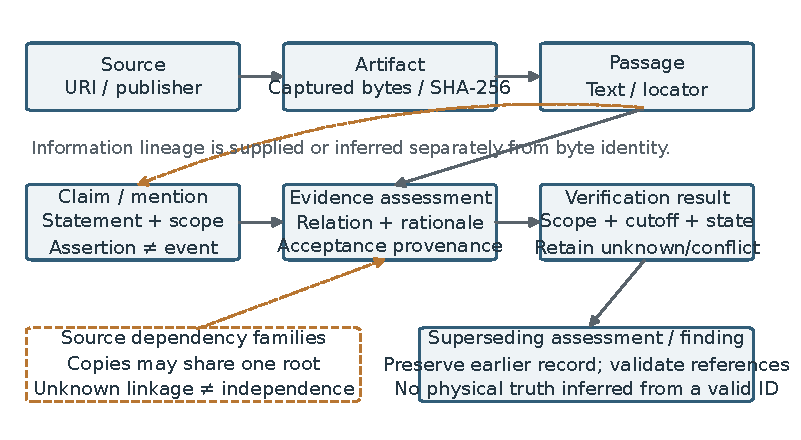
\includegraphics[width=\linewidth]{evidence_provenance.pdf}
\caption{Evidence and provenance relationships. Source assertions, artifact
bytes, extracted passages, and analytical judgments remain distinct. Recorded
lineage and valid locators support inspection without guaranteeing truth or
source independence.}
\label{fig:provenance}
\end{figure}

Local retrieval uses BM25 over supplied passages, searches claim and
counterevidence directions, and respects a capture-time cutoff and query budget.
Results remain unassessed candidates. An assessment constructor checks that its
quoted Unicode-codepoint span equals the passage substring, validates scope and
numeric constraints, and records acceptance provenance. Accepted assessments
require either a human-adjudication label or a validated-rule label with a rule
identifier. This is a structural requirement: the constructor does not consult
an independently validated rule registry. The dedicated claim builder supplies
the latter label programmatically.

The shared verification vocabulary contains seven states:
\code{unverified}, \code{supported_within_scope},
\code{refuted_within_scope}, \code{conflicting_evidence},
\code{insufficient_evidence}, \code{not_verifiable}, and \code{superseded}.
It excludes candidate-only, mistimed, scope-mismatched, or improperly cited
assessments. Verdict thresholds count declared source-lineage identifiers;
separate fields count roots explicitly marked independently confirmed.
These quantities must not be conflated. A physical-fact scope additionally
requires an accepted direct physical evidence basis before support or refutation
can stand. Institutional denials can therefore remain recorded as an official
position while the physical claim remains insufficiently evidenced. This guard
depends on the supplied scope type; it does not independently classify a claim's
epistemic scope.

The curated case package contains 25 claims, 25 selected passages, and 36 accepted
rule assessments. Its current schema~2.3 outputs are 19 supported, zero refuted,
and six insufficient-evidence results. These are program outputs, not accuracy
measurements. The earlier schema~2.0 package produced 21 supported and four
refuted results from 31 assessments, while injecting designated passages and
expected relations into assessment construction. Current code assesses only
retrieved candidates and removes that direct injection, but claims, queries,
passages, scopes, and lineage labels remain curated. The general offline runner
is more restricted: it retrieves candidates and creates no accepted assessments.

Two hand-designed challenges expose semantic failures in the current matcher.
A passage about 26 trees is accepted as supporting a claim about 26 military
occupants, and a sentence negating police arrival is accepted as supporting
arrival. Both receive the fixed branch confidence 0.92. The stored case artifact
also accepts injury and independent-walking passages as support for a claim about
four deserters. Numeric agreement can satisfy the support rule without matching
the predicate; lexical overlap can miss ordinary negation. Moreover, inference
uses the entire passage while the stored citation may be a shorter retrieved
span. Exact quotation therefore does not guarantee that the quotation entails
the assigned relation.

No independent local gold set establishes entailment accuracy or calibrates these
confidence values. The challenges demonstrate failures rather than estimating
their prevalence. FEVER and AVeriTeC motivate evaluating evidence adequacy jointly
with verdict correctness \citep{thorne2018fever,schlichtkrull2023averitec,
schlichtkrull2024averitec}; they provide no substitute for evaluating this system
on independently adjudicated claims. InFact provides an external staged comparator
\citep{rothermel2024infact}, not a measured baseline here.

\section{Event mentions and two temporal layers}
\label{sec:events}

Event reconstruction accepts already typed mentions containing a predicate,
actor and object identifiers, place, evidence references, and temporal metadata.
It does not extract events autonomously from reports, posts, or video. This
boundary differs from supervised span-based extraction, where predicted triggers
and arguments are evaluated against annotated text
\citep{wadden2019dygiepp}. The implemented contribution is conservative
organization of supplied assertions.

Communication mentions use publication timestamps; physical mentions require
supplied earliest and latest event-time bounds to enter their timeline. Missing
or partially bounded physical time is preserved without substituting publication
time. Figure~\ref{fig:dual} presents the two layers. Pairwise interval comparisons
produce before, after, overlap, or unknown relations, with every temporal edge
explicitly marked noncausal. Ordering reports cannot establish that one physical
action caused another.

\begin{figure}[tb]
\centering
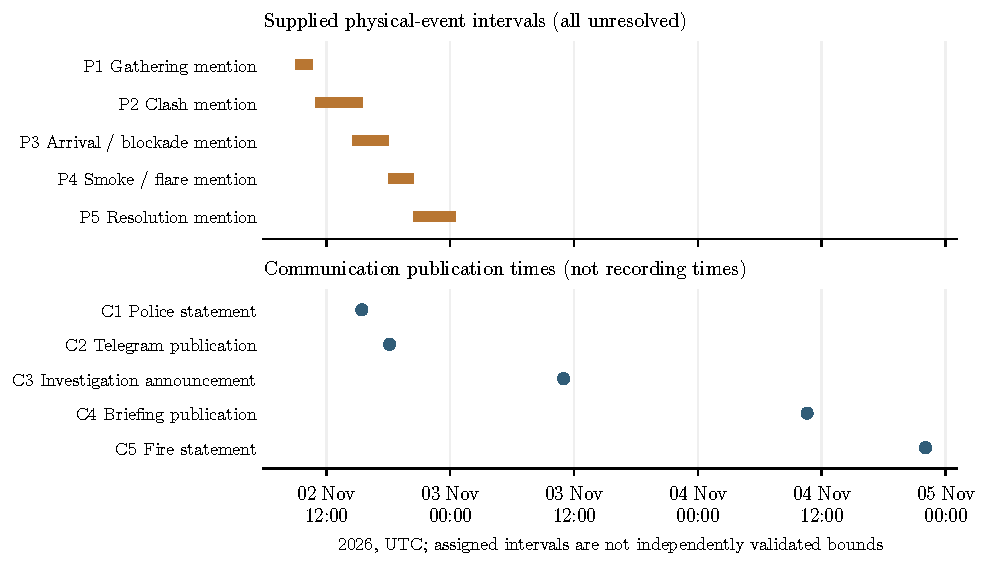
\includegraphics[width=\linewidth]{dual_timeline.pdf}
\caption{Separate communication and physical-event timelines. Publication times
locate communications; analyst-supplied intervals locate reported physical
episodes. Overlapping bounds and unresolved mentions remain visible, and temporal
order carries no causal interpretation.}
\label{fig:dual}
\end{figure}

Exact agreement of normalized predicate, actor identifiers, object identifiers,
and place can produce a reviewable possible-same link, subject to temporal
compatibility and supplied cannot-link constraints. The function never merges
mentions. This restraint matters because similar descriptions can refer to
different event instances, a difficulty emphasized by ECB+
\citep{cybulska2014ecbplus}. Cannot-link constraints preserve analyst-specified
distinctions; they are not independently discovered identity judgments.

The curated timeline contains five physical and five communication mentions.
All ten remain unresolved, with zero possible-same links. Actors, intervals,
participant positions, and qualitative evidence tiers are supplied in the
builder's literal input list. Those tiers describe the asserted evidence basis,
not calibrated confidence or verified physical occurrence. Thus the artifact
demonstrates reproducible temporal organization and explicit uncertainty; its
counts do not measure event-discovery recall or reconstruction accuracy.

\section{Multimodal Evidence Processing}
\subsection{Technical acquisition and derivatives}
Multimodal processing begins with local file identity and technical readability, not scene interpretation. \code{media_pipeline.py} streams SHA-256 calculation, probes media, and can perform strict full-file FFmpeg decoding. The separate video runner adapts downloaded archive manifests, validates local files, creates audio and sampled-frame derivatives, and optionally invokes OCR and ASR. Cache reuse depends on content, parameters, model/configuration and code fingerprints. Atomic writes and stat checks reduce accidental reuse of incomplete outputs. These are implemented engineering controls rather than a claim of forensic authenticity certification.

\begin{figure}[tbp]
\centering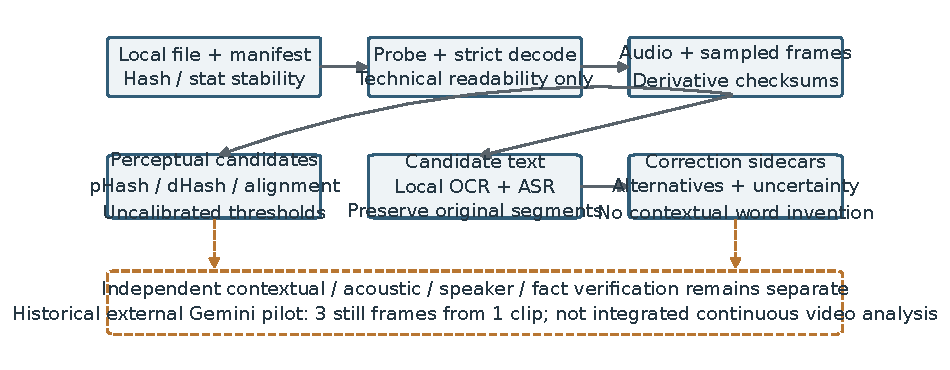
\includegraphics[width=\linewidth]{multimodal_pipeline.pdf}
\caption{Implemented local multimodal pipeline. Technical processing produces inspectable candidate observations. Independent acoustic, contextual, identity and event verification are separate tasks; the historical external three-keyframe Gemini pilot is not part of this automated runner.}
\label{fig:media}
\end{figure}

Sampled frame comparison combines a 63-bit low-frequency DCT perceptual hash and a 64-bit horizontal difference hash. It evaluates full, border-cropped and center-cropped variants, including horizontal mirrors, and excludes low-information frames. The default candidate rule uses Hamming limits of 10 and 12, at least .6 temporally consistent coverage of the shorter analyzed window, three distinct matching frames and hashes, and a two-second span. Nearest-frame offsets and their median deviation describe relative sequence alignment. These exploratory thresholds are not calibrated match probabilities. Similar overlays, static scenes and selection effects can produce false positives; sparse sampling, edits and cropping can produce false negatives. Neither a match nor a nonmatch establishes recording location, event identity, copy direction, or authenticity.

\subsection{Candidate speech and text}
The optional text path uses Tesseract OCR and faster-whisper ASR. OCR outputs word boxes and timestamps linked to frames; ASR outputs timed text segments. Tesseract's established OCR architecture and Whisper's multilingual training provide useful extraction foundations \citep{smith2007tesseract,radford2023whisper}. Their published results do not quantify performance of the exact converted models on Social's Ukrainian, Russian, mixed-language or noisy recordings. Faster-whisper's runtime and decoding settings also need explicit versioning \citep{systran2026faster}.

Historical bulk receipts name CPU/int8 \code{Systran/faster-whisper-small}, revision \code{536b0662742c02347bc0e980a01041f333bce120}, with faster-whisper 1.1.0. A selected seven-asset second pass used \code{mobiuslabsgmbh/faster-whisper-large-v3-turbo}, revision \code{0a363e9161cbc7ed1431c9597a8ceaf0c4f78fcf}. This selection is not a controlled corpus-wide model comparison. Original and alternative text are retained as correction sidecars; ten lexical candidates in that review remain \code{quote_safe=false}. Plausible contextual wording is insufficient grounds for silently filling inaudible speech.

Quotation safety has several separate requirements: text must match the audio, speaker identity must be justified if named, the quotation must preserve context, and factual assertions inside the quotation need their own evidence assessment. The 18-clip benchmark stores ten \code{quote_safe=true} flags, but an AI worker identifier accompanying a ``human acoustic listening'' field does not independently demonstrate a human listener. We report the supplied-reference error arithmetic and recorded flags, not independently verified quotation safety. Unexpectedly higher error in a nominal clean-speech stratum cannot establish a general noise effect: clips, terminology and reference construction differ, with only a few clips per stratum.

\subsection{External model feasibility versus integration}
A historical receipt describes a user-Agy Gemini 3.8 Flash pilot on three still frames from one 15.278-second clip. A full-video attempt was blocked, while the keyframe run returned candidate visual observations. This is feasibility evidence for an external tool invocation, without continuous-video, audio, geolocation, identity, truth or accuracy validation. The current Python runner contains no automatic Gemini/Agy call. Reported token counts are not a measured monetary cost, and outputs from another model are not independent corroboration of the scene.

\section{Autonomous Workflow and Reliability}
\subsection{What the controller actually automates}
The incident orchestrator accepts a typed incident specification, fixed Source Watch audit inputs and resource budgets. In execution mode its code-owned registry can call the existing allowlisted web collector. Seed URLs do not automatically enlarge that registry or its domain allowlist. Newly returned capture manifests can pass through the ingest bridge into a run-local evidence ledger. Optional typed offline inputs can then be processed. Dry-run planning, collection execution, and local analysis are explicit independent options.

The offline runner invokes lineage, retrieval, typed timeline organization, information summaries, supplied conflict inputs, uncertainty scenarios and report checks where compatible inputs exist. It records absent inputs as blocked or not run rather than fabricating them. Retrieval does not invoke the dedicated curated claim-builder's acceptance heuristics. Report generation expects a separately supplied bundle containing findings, evidence records and verification results. Thus a successful controller execution is not evidence that raw sources were transformed autonomously into verified findings. Figure~\ref{fig:workflow} shows the decisive boundary.

\begin{figure}[tbp]
\centering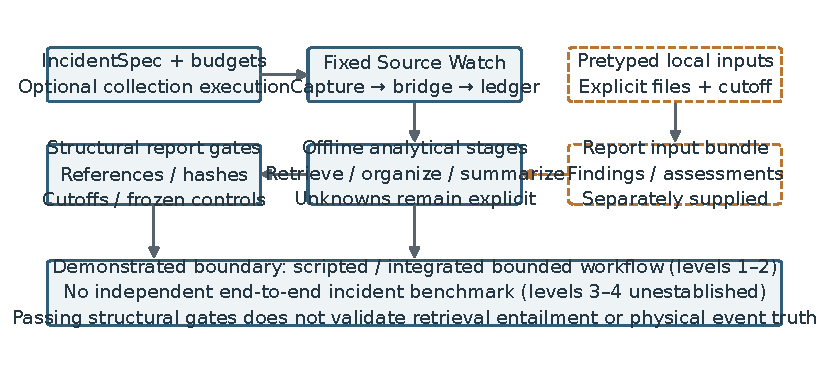
\includegraphics[width=\linewidth]{analysis_workflow.pdf}
\caption{Bounded workflow and automation boundaries. Typed inputs, curated judgments and separately run media analysis enter through explicit interfaces. Structural gates can reject invalid references; they cannot turn a candidate passage into a semantically warranted finding. The end-to-end investigative claim remains unvalidated.}
\label{fig:workflow}
\end{figure}

\subsection{An explicit descriptive autonomy scale}
For this paper, level~0 means manual operation; level~1 scripted processing of supplied inputs; level~2 an integrated automated analytical workflow; level~3 evidence-aware autonomous search and assessment within independently validated tasks; and level~4 independently validated end-to-end analysis on incidents with initially unknown results. This is an author-defined descriptive scale, not a community standard or an ordinal accuracy measure.

Most collectors, local indexing and curated builders operate at level~1. The typed offline runner and limited orchestrator demonstrate level~2 integration. Their semantic inputs and conclusions remain bounded by supplied data and unmeasured inference quality. A separately executed heuristic claim builder does not raise the whole system to level~3; no current result demonstrates level~4. Human or externally validated reference sets are needed during development and evaluation, but this does not imply a human must label every future record in production. Rather, unsupported production tasks must remain unknown or outside the validated operating envelope.

\subsection{Reliability gates and uncertainty}
The evaluation harness checks schema shape, references, time cutoffs, source dependencies, report artifact hashes and frozen synthetic scenarios. It explicitly marks semantic evaluation not evaluated. In particular, 783 passing tests cannot imply 100\% factual accuracy. Structural acceptance provenance such as \code{validated_rule} does not establish that a rule was independently validated. Fixed heuristic confidence values are not calibrated probabilities.

Uncertainty scenarios expose dependence on disputed labels, unknown channel groups, removal/capping assumptions and concentrated observations. Their intervals are scenario bounds conditional on the supplied records, not sampling confidence intervals for population opinion. Incremental dispatch and report differences can identify affected outputs and changed decisions, but do not guarantee that a revised substantive conclusion is true. The engineering priority is transparent failure and inspectability, consistent with reproducible research practices \citep{sandve2013reproducible,wilson2017practices}; semantic reliability remains a separate empirical obligation.

\section{Evaluation}
\label{sec:evaluation}

Evaluation separates computational reproducibility, deterministic contract behavior, descriptive corpus measurements, and semantic correctness. These categories have different reference standards. A byte-identical replay establishes repeatability of a transformation; a negative control establishes rejection of a specified invalid input; neither establishes the truth of a reconstructed event. Table~\ref{tab:evaluation} reports all ten system experiments with their evidence category and remaining limits. Machine-readable values, source hashes, denominators, environment, and commands accompany the paper in \texttt{audited\_evaluation\_metrics.json}; execution logs are retained separately. No fresh collection or model inference was required for these checks.

\begin{table*}[t]
\centering
\small
\caption{System evaluation matrix. ``Evaluated'' denotes the stated bounded measurement, not independent semantic validation. Historical receipts are distinguished from fresh checks.}
\label{tab:evaluation}
\begin{tabularx}{\textwidth}{@{}p{0.07\textwidth}p{0.19\textwidth}XX@{}}
\toprule
ID & Experiment & Evidence and observed result & Evaluation boundary \\
\midrule
E1 & Reproducibility & Fresh hash checks, exact-graph replay, saved-draw arithmetic, and four 25-draw prefixes agree. & No fresh recrawl; full 9,999-draw generation is a historical replay receipt. \\
E2 & Data collection & Saved historical/expanded counts and missingness independently recomputed. & Integrity and coverage description; platform completeness and relevance recall unknown. \\
E3 & Duplicate detection & Exact sweep: 369 qualifying pairs; 367 retained by legacy candidates; two misses, zero extras. & Conditional finite-corpus candidate recall; no semantic duplicate gold. \\
E4 & Coordination detection & Saved 16-test family: raw $p=.0001$, Holm $p=.0016$; bounded prefixes reproduce. & Conditional exploratory nulls; organic-control specificity and attribution unmeasured. \\
E5 & Evidence retrieval & Captured-corpus retrieval and reference controls exercised by offline tests. & Curated/known inputs; no blind open-web retrieval benchmark. \\
E6 & Claim verification & Abstention, conflict, cutoff, and lineage contract controls pass. & No independent semantic accuracy or entailment score; counterexamples remain material. \\
E7 & Event reconstruction & Typed event organization and synthetic timeline/reference invariants checked. & No autonomous raw-event discovery or independently adjudicated chronology score. \\
E8 & Video/ASR & Historical supplied-reference arithmetic: 185 errors/415 words, 44.58\% micro WER. & Selected clips; independent reference listening provenance not established. \\
E9 & End-to-end workflow & Two clean retrieval-only repeats remain partial/unverified; dangling-event negative control fails. & Two candidates, no accepted support, no generated report; not a blind incident evaluation. \\
E10 & Runtime/resources & Fresh offline suite: 7.84\,s wall, 328,320\,KiB maximum RSS; bounded analytical audit also measured. & Partial local workloads; no current GPU benchmark, API cost, or full-run throughput. \\
\bottomrule
\end{tabularx}
\end{table*}

The fresh full repository suite returned 783 passed tests and 16 passed subtests, with no failures. Pytest reported 7.41\,s; an external resource measurement recorded 7.84\,s wall time and 328,320\,KiB maximum resident memory, exiting successfully. The interpreter was the repository virtual environment's Python 3.13.14 on Linux/x86-64. These counts describe regression coverage, not an accuracy denominator. Six frozen synthetic controls also passed, covering a known microcase, single-root copy fanout, contradictory testimony, correction cutoffs, incomplete evidence, and reused video. Their expected states are known by construction. They are useful release gates without being blind observations of incident truth.

For collection accounting, direct parsing reconciled 23,350 historical publications with 1,408 selected relevant records and 1,384 texts eligible for similarity analysis. The historical 459 missing raw texts and 49 absent view counters belong to all publications; neither is missing among the relevant subset. The remaining 24 relevant texts are shorter than the 80-character eligibility threshold. The expanded snapshot contains 23,386 publications and 1,438 relevant records. These versions are distinct analysis frames. The exact graph and conditional timing tests use the historical frame; a lineage document's assignment of that graph to the expanded frame was rejected against its recorded input hashes. Such checks address denominator integrity without establishing sampling representativeness~\cite{Olteanu2019,VicentePaula2023}.

The duplicate experiment recomputed the entire eligible exact graph using the production five-character shingle definition and 64-bit intersection arithmetic. At Jaccard thresholds .60, .75, and .90, exact cross-channel totals were 369, 288, and 213; legacy retrieval retained 367, 288, and 213. Thus candidate recall at .60 is $367/369=99.45799458\%$, conditional on the 1,384 eligible historical texts. Eighteen same-channel qualifying pairs are excluded by the graph definition. Both missed cross-channel edges exceed 30 minutes, so the observed short-lag counts remain 134 within ten minutes and 198 within thirty minutes, each now divided by 369. Figure~\ref{fig:copy} presents this distinction between candidate retrieval and exact measurement. Shingle sketching supplies a retrieval mechanism, not semantic identity or source dependence~\cite{Broder1997}.

\begin{figure*}[t]
\centering
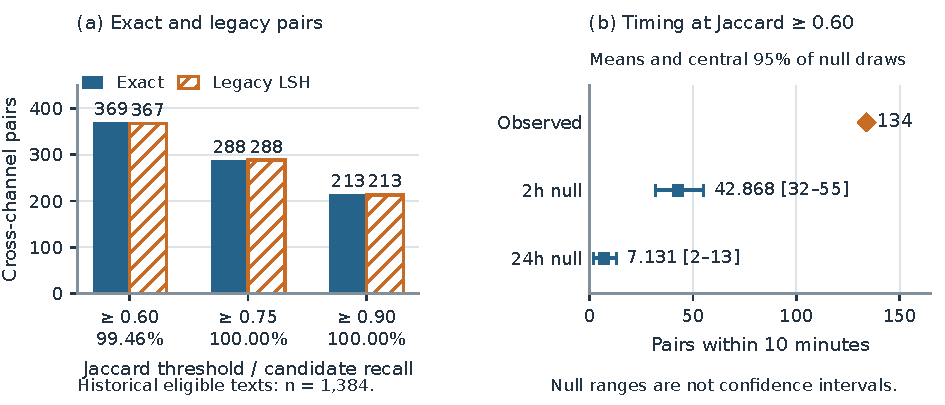
\includegraphics[width=\textwidth]{information_analysis.pdf}
\caption{Finite-corpus similarity retrieval and conditional copy timing. Left: exact versus legacy retained pairs, with recall at each threshold, among 1,384 eligible historical texts. Right: 134 observed pairs at Jaccard $\geq .60$ within ten minutes versus the two saved conditional-null means. Whiskers show the central 95\% of 9,999 randomization draws, not confidence intervals. All timing counts use the fixed 369-edge graph. Sources and hashes are retained in \texttt{data/figure\_data/information\_analysis.json}.}
\label{fig:copy}
\end{figure*}

For coordination, every saved draw was reread and all sixteen summary rows were recomputed, including means, quantiles, upper-inclusive tails, and multiplicity adjustment. With 9,999 draws, all recorded exceedance counts are zero; the plus-one Monte Carlo value is $(0+1)/(9999+1)=.0001$, and Holm adjustment over this declared family gives .0016~\cite{Phipson2010,Holm1979}. A fresh replay reproduced the first 25 draws of each of four models using seed 20261106. This audit did not regenerate all draws. Timing permutations assign one rotated time to each graph node, shared across its edges. Consequently, edges are not treated as independent trials. Departures from these conditional backgrounds do not establish intent, inauthenticity, an organizer, or specificity against matched benign events~\cite{Pacheco2021,Nizzoli2021,Magelinski2022}.

Semantic evaluation remains more limited. The narrative comparison pairs rules with Claude labels on forty selected test posts, rather than independent human adjudication; its agreement statistics cannot validate stance accuracy. Evidence retrieval operates over a captured corpus, and lexical ranking does not establish passage entailment~\cite{RobertsonZaragoza2009BM25}. Curated claim regression checks and synthetic counterexamples are reported as such. Typed event records organize supplied assertions; structural validity does not demonstrate discovery of the underlying physical events. Likewise, the historical ASR error calculation uses supplied reference strings whose independent listening provenance was not established. Its 44.58\% micro WER is descriptive arithmetic for those clips, not a blind corpus-wide recognizer benchmark.

The fresh workflow smoke artifact records two repeat retrieval-only runs with two candidates, an unverified claim, zero accepted support assessments, and no report. A third run deliberately introduces a dangling event evidence reference and correctly fails the evaluation gate. Equal semantic projections across the clean repeats establish bounded repeatability, while their partial status identifies unfinished stages. The combined analytical audit took 4.8317\,s and 1,032,620\,KiB maximum RSS, including corpus loading, exact comparison, saved-draw checking, prefix replay, and graph/bin reconstruction. These resource measurements exclude collection, production ASR, external models, and subsequent auxiliary checks. No current GPU timing or monetary API cost was measured. Independent incident-level evidence, event, and report accuracy therefore remain unmeasured outcomes rather than inferred benefits of a passing software suite.

\section{Real-World Application: A Bounded Digital-Trace Investigation}
\label{sec:application}
The Petropavlivska Borshchahivka application illustrates how the software handles an information-rich local conflict without supplying a definitive reconstruction of that conflict. The incident and subsequent reporting span 2--9 November 2026; particular collections have narrower windows. The separate case manuscript discusses substantive claims \citep{pylypenko2026case}. Here the application is organized by analytical handoffs: what entered each component, what it produced, and what remained unresolved. It is a demonstration workload rather than a new independent incident benchmark.

\subsection{From a purposive panel to a frozen analysis frame}
The historical Telegram panel has 241 monitored channel identifiers and 23,350 collected posts, with 1,408 selected as relevant from 159 channels. It is a targeted panel rather than a census. The relevant text and view-counter fields are nonmissing in that frame. The sum of their snapshot view counters is 115,931,014; this is neither unique audience size nor a measure of persuasion. Collection age, repeated exposure, forwarded material and unavailable users prevent such interpretations. Reporting the large sum without its counting rule would exaggerate what the system measures.

A later merged frame contains 23,386 posts, 1,438 relevant records and 158 relevant channels. It has a different SHA-256 from the historical file. Both frames are useful for different analysis receipts, but their denominators cannot be substituted. The publication audit recovered this distinction by parsing the actual JSONL and comparing its digest with experiment inputs. It also found a lineage report that assigned the 369-edge exact graph to the merged corpus despite the experiment's historical input hashes. We retain the historical documents and correct the attribution in the new paper's evidence matrix. This demonstrates both the usefulness of machine-readable provenance and the need to check whether its assertions are correct.

\subsection{From text candidates to reproducible information signals}
Of the 1,408 relevant records, 1,384 have cleaned text at least 80 characters long. Exhaustive cross-channel Jaccard comparison produces 369 edges among 357 posts and 113 channels. Legacy MinHash output contains 367 of those edges. The two omitted edges have lags exceeding thirty minutes, so their inclusion changes the graph denominator without changing the short-lag numerators. This result is a concrete systems lesson: approximate retrieval can be evaluated against an exact bounded universe before inferential statistics are interpreted.

On the exact graph, 134 pairs occur within ten minutes and 198 within thirty minutes at Jaccard .60. The two-hour rotation null gives a ten-minute mean of 42.868 pairs and central draw range 32--55, compared with a 24-hour-model mean of 7.131 and range 2--13. The difference between these baselines shows how conditioning on shared activity changes the comparison. Both retain departures in this dataset; neither identifies who controlled the channels or whether the copying was deceptive. The audit's fresh prefix replay and arithmetic checks assess computation, while the absence of matched organic waves limits substantive specificity.

The visible-forward network is smaller and measures a different relation: 69 endpoint channels, 60 directed channel-pair edges and 65 observed forward events. Isolated channels do not appear in that edge-induced graph. Text similarity is not substituted for explicit forward attribution, and centrality is not used as proof of organizational command. Fifteen six-hour narrative bins include two empty bins and a final partial bin. The short, nonstationary, shared-event series and weak label validation do not support causal time-series claims. The implementation accordingly withholds a Granger-causality interpretation in the inspected network analysis.

\subsection{From selected discussions to audience limits}
The comment workload contains 39,598 records in 533 selected threads, with 39,459 available author identifiers and 12,797 pseudonymous authors. The 139 records lacking an author identifier cannot enter known-author analyses in the same way. The thread set was chosen partly for discussion activity. Pagination completeness within these threads does not make them representative of all Telegram comments, silent readers or the Ukrainian public. One author may contribute many observations; comment-weighted and author-weighted estimates therefore answer different questions.

Reaction capability was checked separately on ten comments from three threads. It establishes that a contemporary MTProto snapshot can expose reaction detail for those accessible messages, not a measured emoji distribution across all 533 historical threads. Social's audience contracts can preserve such snapshots and supplied target-aware labels, but the present evidence does not justify automatically generated percentages of anger, support or toxicity. The application illustrates an important engineering constraint: collecting a large discussion corpus is not equivalent to having validated semantic analytics for it.

\subsection{From institutional records to scoped evidence states}
The dedicated claim builder supplies 25 selected propositions and 25 selected passages. Current output has 19 supported-within-scope and six insufficient-evidence results, with no refuted-within-scope results. These states can document that an institution made a statement, while leaving the physical allegation it discusses unresolved. In particular, official denials are retained as official positions rather than independent proof that a physical event did not occur. Source roots and scope types remain supplied interpretive metadata; their existence in a schema does not verify independence or scope correctness.

The application also exposes the limit of lexical relation rules: passages about injuries were accepted for a proposition about deserters because the number matched. That is a material failure despite valid references and numeric agreement. It prevents treating the 19 supported outputs as 19 independently established truths. The post-audit revision in Section~\ref{sec:rule-v2} withdraws those acceptances and also withholds the court-bail claim, whose passage does not name the person, leaving 18 supported and seven insufficient-evidence results. Those 18 are likewise not independently established truths. The general runner takes the more conservative path of candidate retrieval without accepted assessments. These are different code paths, and the paper does not transfer the curated builder's output inventory to the general workflow.

\subsection{From media bytes to candidate observations}
Historical archive receipts list 775 downloaded-verified source-post rows corresponding to 607 unique SHA-256 assets. A strict technical index reports all 607 as decodable, totaling 9,472,884,834 bytes. Extraction receipts describe 8,679 frames, audio available for 602 assets and absent for five, and approximately 12.04 summed hours of container duration. Container duration is not speech duration; these historical measurements were not rerun for this publication.

Bulk ASR produced 10,872 candidate segments across 558 complete text results, 44 no-segment results and five assets without audio. The 18 selected reference clips yield 185 errors over 415 reference words. These inventories demonstrate scale of technical processing and potential error, not authenticity, speaker identity or acoustic verification. A visual-overlap candidate can guide analyst inspection but cannot establish that a clip depicts the local allegation attached to it. The application ends with structured unknowns wherever source authenticity, location, physical events or semantic entailment remain unvalidated. Its practical value is a traceable analytical workspace rather than a final adjudication of the conflict.

\section{Discussion}
\subsection{Practical value of integration}
The main advantage of Social is continuity between otherwise separate analytical tasks. An analyst can inspect a frozen acquisition frame, follow a normalized record to available source material, compare a candidate copy graph against an exact computation, examine a conditional null, and retain unresolved evidence in a report-oriented workflow. The framework's value is reduced ambiguity about which record, assumption and transformation produced an output. We have not measured analyst time savings or compared final investigation quality against expert-only work, so these benefits are architectural affordances rather than established productivity effects.

Several design choices are deliberately modest. JSONL and SQLite are inspectable and practical for a single researcher. Deterministic rules are easier to replay than an unconstrained agent, and local media processing avoids sending every private asset to a cloud model. However, transparency of a rule does not make it semantically correct: the numeric-predicate counterexample is a direct illustration, and narrowing that rule after the audit did not make it a validated entailment model. The safest general runner currently abstains from acceptance; the more ambitious curated path exposes how misleading structural completeness can become when acceptance labels are trusted too readily.

\subsection{Answers to the research questions}
RQ1: acquisition, snapshots and the typed offline workflow are integrated in part, while media processing, several collectors and curated builders remain separately run. RQ2: reference, hash-format, cutoff and supersession invariants are enforced; entailment, authenticity and source independence are not. RQ3: the exact graph, saved randomization summaries and seeded prefixes reproduce on frozen inputs. RQ4: communication and physical timelines are kept separate, but physical intervals are supplied by an analyst. RQ5: numeric-predicate and negation failures passed the software gates until the rule was narrowed, and broader semantic error remains unmeasured. RQ6: a bounded level-2 workflow is supported; independently validated investigation is not.

\subsection{Lessons for evidence-grounded software}
First, provenance is a set of claims requiring validation, not merely a collection of hashes. A hashed lineage document can assign a result to the wrong corpus. Second, reliability is multidimensional: test success, correct arithmetic, citation integrity, semantic entailment and event truth can diverge. Third, autonomy should be assigned to a particular execution path and task. A video pilot, a manual event list and a retrieved passage bundle cannot be combined rhetorically into an independently validated autonomous investigator. Fourth, honest unknowns are useful outputs. They preserve what additional evidence would be necessary and prevent a plausible completion from replacing an absent observation.

The next research priority is independent semantic evaluation on separated incidents and source families, rather than more elaborate model orchestration. A frozen gold set can support model development and regression evaluation without requiring manual review of every future incident, but deployment claims must remain bounded by demonstrated transfer. An LLM-only or multi-model baseline would require matched inputs, tasks and budgets. No such comparison was executed here, and model agreement would still not provide independent corroboration.

\section{Limitations and Threats to Validity}
\subsection{Internal and construct validity}
The evaluation is uneven by design because the implementation is uneven. Exact shingle-graph reproduction measures a well-defined computation, while most semantic tasks lack an independent reference. The current claim builder is conditioned on selected propositions, queries, sources and scope types. Removed direct expected-label injection is a meaningful improvement, but does not transform this corpus into a blind benchmark. Hand-designed counterexamples establish that a failure is possible, not its frequency. The later stress test shares this limit: its cases were written after the failures were known, by the same AI system that revised the rule. The same distinction applies to frozen synthetic report and event controls.

Constructs are particularly vulnerable to substitution. Lexical themes are not stance; reaction counts are not endorsement of every proposition; repeated text is not independent testimony; state-associated infrastructure is not operational ownership; a technically valid clip is not a verified scene; and exact quotation offsets are not entailment. Supplied source-lineage roots can prevent known copy fanout, but unknown dependencies remain. The verification aggregator's physical-fact protection depends on correct supplied scope labels, so a misclassified scope can still overstate a conclusion.

\begin{table}[tbp]
\caption{Reliability layers and claims that remain unestablished.}
\label{tab:reliability}\small
\begin{tabularx}{\linewidth}{@{}p{27mm}X X@{}}\toprule
Layer & Evidence available & Not established by it\\\midrule
Software & Passing regression suite, schemas, reference and cutoff gates & Complete test coverage, security certification, semantic correctness\\
Statistical & Replayed exact graph, saved draws, seeded prefixes, Holm arithmetic & Benign-event specificity, campaign attribution, causal influence\\
Evidence & Captured bytes, locators, declared lineage, supersession & Source truth/authenticity, independent roots, passage entailment\\
Multimodal & Decode/extraction receipts, supplied-reference text comparison & Reliable identity/location/time, independent quotation safety\\
Report & Artifact hashes, citation/reference and numerical checks & Factual completeness, all unsupported claims detected\\\bottomrule
\end{tabularx}
\end{table}

\subsection{External and statistical conclusion validity}
Only one real incident supplies the central workloads. The sampled channels, selected threads, curated statements and accessible media do not form a representative frame. Deleted material, moderation, ranking, search selection and platform restrictions can affect both observed volume and content. No matched organic event set estimates false-positive coordination rates. Reported randomization departures depend on exchangeability within chosen strata; none establishes population prevalence or causal information effects. Shared nodes and copied sources also preclude treating graph edges or repeated assertions as independent observations.

The 18 ASR clips are selected and small. Reference strings, acoustic strata and quotation flags lack independently established adjudication provenance. Error-rate differences across strata can reflect lexical difficulty and selection rather than noise alone. The seven-asset larger-model review is not a paired corpus-wide performance trial. Perceptual thresholds have no labeled match/nonmatch benchmark. Negative media matching cannot establish that recordings depict different events.

\subsection{Automation, source and temporal validity}
The orchestrator integrates a limited collection adapter and pretyped analysis, not all platform collectors. Physical mentions and some report content are curated. No independent incident-level end-to-end benchmark measures source discovery, claim extraction, evidence adequacy, physical-event reconstruction and final report correctness together. Internal AI-agent review is not independent human peer review; worker names and acceptance labels do not establish human involvement. Numeric confidence constants are not calibrated uncertainty.

Capture time and evaluation time cannot reconstruct what a website showed earlier. HTTP/TLS failures leave coverage gaps. Some historical raw manifests or private derivatives are absent from the tracked artifacts, limiting replay. A report-linked Source Watch capture and a different locally available capture must remain distinct even if headline counts coincide. Publication, capture, recording, claimed event and evaluation times must not be silently substituted. Legacy case-specific time handling also limits reuse across seasons and locations.

\subsection{Privacy, ethics and release limits}
Public accessibility does not eliminate privacy risk. Pseudonymous identifiers can still support linkage, while verbatim comments, detailed timelines and cross-platform combinations may expose individuals. This publication package contains aggregate measurements, synthetic challenges, code references and hashes rather than raw commenter identifiers, phone numbers, authentication material or bulk comment text. It does not claim that all repository artifacts are safe for unrestricted release. Raw-data sharing requires a separate privacy and platform-terms review. The Berkeley Protocol and social-data bias literature support keeping acquisition ethics and evidentiary quality separate from mere technical accessibility \citep{berkeleyProtocol2022,Olteanu2019}.

\section{Conclusion}
Social implements a substantive collection of interoperating analytical components: source-specific acquisition, versioned snapshots, information-wave measurements, linked evidence accounting, bounded retrieval, typed event organization, local media processing and structural report gates. Frozen-input checks reproduce similarity and conditional-randomization outputs, while explicit challenges reveal semantic failures that a large passing test suite does not exclude. The system is best characterized as an evidence-grounded automated analytical framework with uneven component validation and bounded workflow autonomy. Its practical contribution is inspectable computation and retained uncertainty. Independently validated fact verification, physical-event discovery and general end-to-end incident reliability remain unestablished.

\section*{Reproducibility and Research Artifacts}
The evaluated software is frozen at \code{f0e9d0d67422b0c286a2cb9e7d4e935a833a9533}. New publication files are separate from that baseline and identify their producer commands. The companion package includes the architecture audit, scientific claim--evidence matrix, environment snapshot, experiment manifest, aggregate evaluation data, vector-figure sources and inputs, synthetic workflow/counterexample artifacts, and LaTeX/BibTeX sources. Exact input SHA-256 values bind results to historical or expanded corpora. Timing tests record seed 20261106 and 9,999 saved draws; this publication replays 25 draws per model and recalculates all saved summaries. Stochastic prefix agreement is distinct from a fresh full simulation.

The repository's contract requirements are ranged, while its optional local video requirements pin faster-whisper 1.1.0, PyAV 18.1.0 and requests 2.34.2. There is no unified installation lockfile. The audit environment and rendering environment are separately recorded; the measured test run uses Python 3.13.14, while figure/PDF preparation uses system Python 3.12.3. A clean-environment installation and complete historical platform recollection were not evaluated. Reproducibility practices follow the principle of retaining data, transformations, parameters and intermediate results \citep{sandve2013reproducible,wilson2017practices}; the private corpus prevents unrestricted third-party replay of all stages. FAIR principles motivate reusable metadata without implying that privacy-sensitive data must be openly downloadable \citep{wilkinson2016fair}.

\section*{Data and Code Availability}
The project repository is \url{https://github.com/cyberdid/social}; access was private at the time of this audit. Public availability or a future release is not asserted. Raw Telegram/comment/media data and credentials are not distributed with this paper. Privacy-preserving aggregate and synthetic supplementary materials accompany the manuscript in the publication directory and can be considered separately for release. The distinct case-study manuscript remains a project draft with unconfirmed public publication status. Source availability, computational repeatability and independent semantic validation are separate limitations.

\section*{Author Contributions}
Oleksandr Pylypenko led the conceptualization, system design, research design and implementation direction; supervised analysis and interpretation; and directed manuscript preparation. This statement does not imply personal execution of every software or computational step. The author is responsible for final review and approval.

\section*{Funding and Competing Interests}
This research received no external funding. The author declares no competing interests, consistent with the latest confirmed project manuscript declarations.

\section*{Generative AI Disclosure}
Generative AI tools assisted software development, documentation, computational auditing, literature organization, manuscript drafting and editing. Separate AI-agent critiques supported the publication review. They are not independent human peer review, gold labels or corroborating evidence. A historical external Gemini keyframe pilot is described only within its documented scope; no new paid model inference was used for the reported publication-audit computations. The author retains responsibility for checking, interpreting and approving the manuscript and its research artifacts.

\bibliographystyle{unsrtnat}
\bibliography{references}
\end{document}
